\chapter{The Proposed Centralized Solution}\label{cha:existingSystem}

Question~\ref{PS:Q:HowWellDoWeScale} in the problem statement asks for a comparison between the decentralized solution and the current system at Siemens on different levels. In order to make these comparisons, basic assumptions about the current system at Siemens must be in place. 

Ideally, for us to compare the two systems on equal terms, both systems should be implemented in the same environment. However, since we do not have access to the environment where the current system at Siemens is implemented, we have chosen to build our own version of the current Siemens system, in the same environment as the decentralized system.

This version of their system, from now on referred to as the centralized solution, is built from what Siemens has told us about the current Siemens system. The goal of this version of their system is to create a foundation for a comparison between the decentralized solution and the current Siemens system, by ruling out the environment as a parameter. Since we don't have access to the Siemens environment, we aim to close some of the theoretical gap between the current Siemens system and the decentralized solution, using the centralized solution. As a result, we aim to compare the centralized solution with the decentralized solution.

However in order to completely answer question~\ref{PS:Q:HowWellDoWeScale}, and compare the decentralized solution with the current Siemens system, another comparison must be introduced: A comparison between our centralized solution and the current Siemens system. This comparison is theoretical and based solely on assumptions and what we know about the current Siemens system. 

The thesis motivation (\cref{sec:ThesisMotivation}) describes a brief overview of the current system at Siemens. This chapter gives a detailed description of the key component of the current Siemens system: The regulation algorithm. Furthermore the chapter describes the centralized solution followed by a theoretical comparison between the centralized solution and the current Siemens system. 

%Only built for comparison/testing purposes

%Logic view. What classes are where?

%Data Objects

\section{Regulation algorithm}\label{sec:regAlgorithm}

The regulation algorithm is a key component of the system and it is where new setpoints are calculated. Since the purpose of this thesis is not to improve any regulation algorithms, the regulation algorithm has been considered a black box in development of both the centralized and the decentralized solution. What is important to this thesis is that the algorithm used is the same in both the centralized and the decentralized solution, to make sure the two systems are compared on the same terms. 

To get as realistic a picture of the system as possible of the regulation algorithm, we tried to gain access to the algorithm Siemens currently use, but due to the regulation algorithm at Siemens being a commercial secret, this was not possible.

\begin{figure}
	\centering
	\begin{tikzpicture}[
	point/.style={inner sep=0pt}, %circle,minimum size=2pt,fill=red},
	textNode/.style={inner sep=2pt},
	hv path/.style={to path={-| (\tikztotarget)}},
	vh path/.style={to path={|- (\tikztotarget)}},
	skip loop h/.style={to path={-- ++(0,#1) -| (\tikztotarget)}},
	skip loop v/.style={to path={-- ++(#1,0) |- (\tikztotarget)}},
	graphs/every graph/.style={edges=rounded corners}
	]
	
% Place nodes
\matrix[row sep=1.5cm,column sep=.5cm] {
	\node [point]  		(p1x1)	{}; &&
	\node [rectangle]	(Turbine)		[draw, label=above:Turbine, text width=50pt]	{Cur.prod. Max.prod}; &&
	\node [point]  		(p1x3)	{}; \\
	
	\node [point]  		(p2x1)			{}; &&
	\node [textNode]	(HPPP)		 	{Reg.algorithm}; &&
	\node [textNode]	(Setpoint)	{Setpoint}; \\

	\node [textNode]  (gSetpoint)										{Global setpoint}; &&
	\node [rectangle]	(Data)			[draw, text width=50pt] {Cur.prod  Max.prod};\\
};

\node [textNode,right of=Data] {~~~~~~~~~~~~~~~~~\textbf{$\cdot$}nTurbines-1};
	
\graph[use existing nodes]{
	Turbine ->[skip loop v=-3.1cm] HPPP -> Setpoint ->[vh path] Turbine;
	gSetpoint.east -> HPPP;
	Data -> HPPP;
};

\end{tikzpicture}

	\captionsetup{format=plain,font=footnotesize,labelfont={bf,defaultCapFont},labelsep=quad,singlelinecheck=no}
	\caption[Regulation algorithm input/output parameters]{
		\label{fig:ioRegAlg} 
		\footnotesize{%
			Input/output parameters of the regulation algorithm.
		}
	}
\end{figure}

With the algorithm being a black box, the input/output parameters of the algorithm was studied to provide the correct communication circumstances for the algorithm. \Cref{fig:ioRegAlg} presents a simple input/output overview of the algorithm. Input/output parameters of the algorithm are as follows:

is given a global setpoint and the state of all turbines, from which setpoints for all turbines are calculated (see \cref{sec:calculateSetpoints} for specific explanation of the centralized regulation algorithm). Each turbine are then given a setpoint, which is used to change state of the turbine. The state of the turbine is represented using the following two parameters:

\begin{description}
	\item The \textbf{global setpoint} of the wind farm. This is the production goal of the wind farm. Which means all turbines combined should produce.
	\item The \textbf{setpoint} of each turbine, calculated from the regulation algorithm. 
	\item The \textbf{current production} of the turbine.
	\item The \textbf{maximum production} of the turbine. In real-life, this parameter is amongst others determined from the wind conditions around the turbine.
\end{description}

This input/output parameters of the regulation algorithm is of cause simplified. The current system at Siemens has many more but for purpose of this thesis, this is enough. 



\section{Regulation cycle}\label{sec:currentSystemCen} 

The first area studied when building the centralized solution, was building the frames for the regulation algorithm (see \cref{sec:regAlgorithm}), meaning how to communicate the input/output around the system. 

The regulation cycle of the Park Pilot loops infinitely. This section describes the centralized solution through explaining how a single regulation cycle works.

\subsection{Get turbine states}\label{sec:getTurbineStates}

In order for the Park Pilot to calculate turbine setpoints, the Park Pilot must have the state of all turbines.

\begin{figure}
	\centering
	\begin{sequencediagram} %Created using pgf-umlsd
		\newthread{parkPilot}{:Park Pilot}
		\newthread{turbineDataReplier}{:Turbine Data Replier}
		\newinst{turbine}{:Turbine}
	
		\begin{sdblock}{each turbine}{}
			\mess[1]{parkPilot}{sendRequest}{turbineDataReplier}
			\begin {call}{turbineDataReplier}{readData()}{turbine}{return data}
			\end {call}
			\mess[1]{turbineDataReplier}{sendReply}{parkPilot}
		\end{sdblock}				
	\end{sequencediagram}

	\captionsetup{format=plain,font=footnotesize,labelfont={bf,defaultCapFont},labelsep=quad,singlelinecheck=no}
	\caption[First part of the regulation cycle]{
		\label{fig:getStatesOfTurbines} 
		\footnotesize{%
			First part of the regulation sequence: Getting the state of all turbines.
		}
	}
\end{figure}

A simple overview of the first part of the regulation sequence is presented on \cref{fig:getStatesOfTurbines}. This part of the algorithm is implemented using the RTI Connext Request-Reply implementation~\cite{rtiConnextUsersManual}. The three primary objects of this part of the algorithm are:

\begin{description}
	\item [Park Pilot] The Park Pilot running the regulation algorithm. This object requests the data from all turbines and calculates setpoints when states has been received.
	\item [Turbine Data Replier] The replier object, instantiated on every turbine. Handles the request and sends a reply.
	\item [Turbine] The underlying turbine object, instantiated on every turbine. Interface to the Turbine, which handles communication with the underlying database with simulation data.
\end{description}

The Park Pilot sends a request to a specific topic and then waits until it has received a reply from all the turbines subscribing to this topic, which in our case is all turbines. In a real-life implementation of the system, a timer should be implemented to determine how long to wait for the replies, and maybe even mark a turbine as offline, if a given turbine does not reply within that time period. However, since this is only a prototype for data comparison purposes, this functionality has not been implemented. The request message, sent from the Park Pilot, contains the cycle time, which is only used for data logging purposes (i.e. not used by the turbines).

The Turbine Data Replier is instantiated with the Turbine object and runs on every turbine. After instantiation, the Turbine Data Replier goes into an infinite loop which first waits infinitely for a request, reads turbine data from the Turbine object and finally sends a reply containing the data to the Park Pilot. Ideally, the Turbine Data Replier object should have been implemented as a listener on the request topic using RTI Connext SimpleReplier~\cite{rtiConnextUsersManual}. However, we could not get it to work using the SimpleReplier but waiting infinitely for a request works just as well for our purpose.

The Turbine object is the interface to the actual Turbine. The primary functionality of this object is to change state when a new setpoint is assigned to the object. Furthermore it reads data from the underlying MongoDB database. 

\subsection{Calculate setpoints}\label{sec:calculateSetpoints}

When the Park Pilot has received the states of all turbines the setpoints for all turbines are calculated. Since we don't have access to Siemens' regulation algorithm (see \cref{sec:regAlgorithm}), we have developed our own simple regulation algorithm.

Our regulation algorithm works by first determining how many turbines that are available for production. This is done going through every turbine, checking if they currently hit their maximum production capacity. If a given turbine is producing at maximum capacity, a greater load cannot be assigned to it and the available turbine count is reduced. 

Next the setpoint for every turbine is calculated. This is simply done by dividing the global setpoint for the entire park with the number of available turbines. If this new setpoint is higher than the maximum capacity of a given turbine, the turbine is set to produce at maximum capacity. If this happens, a gab between the maximum capacity and the calculated setpoint is left unhandled, and the wind farm is under-producing until the next cycle, where a new set of setpoints are calculated, with one less available turbine. Hence this gap will eventually be closed unless the maximum capacity of the entire park is reached.

\subsection{Send setpoints}

\Cref{fig:sendSetpoints} presents a simple overview of the last part of the algorithm. This part of the algorithm is implemented using RTI Connext Publish-Subscribe implementation~\cite{rtiConnextUsersManual}. The primary objects are:

\begin{description}
	\item [Park Pilot] Explained in \cref{sec:getTurbineStates}.
	\item [Turbine Outlet] The Park Pilots implementation of a given turbine. Onene of these objects instantiated on the Park Pilot for each turbine in the park. Writing data to each turbine is handled from this object.
	\item [Setpoint Listener] The listener object called when when a new setpoint is published. One of these objects are instantiated on each turbine.
	\item [Turbine] Explained in \cref{sec:getTurbineStates}.
\end{description}

After calculating the setpoints (\cref{sec:calculateSetpoints}), the Park Pilot sends a new setpoint to each turbine. The Park Pilot sets the setpoint of the Turbine Outlet before publishing the Data.

\begin{figure}
	\centering
	\begin{sequencediagram} %Created using pgf-umlsd
		\newthread{parkPilot}{:Park Pilot}
		\newinst{turbineOutlet}{:Turbine Outlet}
		\newinst{setPointListener}{:Setpoint Listener}
		\newinst{turbine}{:Turbine}
	
		\begin{sdblock}{each turbineOutlet}{}
			\begin {call}{parkPilot}{setSetpoint()}{turbineOutlet}{}
			\end {call}
			\begin {call}{parkPilot}{publishData()}{turbineOutlet}{}
				\mess[1]{turbineOutlet}{write}{setPointListener}
				\begin {call}{setPointListener}{setSetpoint()}{turbine}{}
				\end {call}
			\end {call}
		\end{sdblock}				
	\end{sequencediagram}

	\captionsetup{format=plain,font=footnotesize,labelfont={bf,defaultCapFont},labelsep=quad,singlelinecheck=no}
	\caption[Last part of the regulation cycle]{
		\label{fig:sendSetpoints} 
		\footnotesize{%
			Last part of the regulation sequence: Sending setpoints to all turbines.
		}
	}
\end{figure}

The main purpose of Turbine Outlet object is to register and publish setpoints to each turbine. Upon instantiation, the Turbine Outlet registers the turbine id as a RTI Connext key~\cite{rtiConnextUsersManual} to the setpoint topic and saves the handle object. Saving the handle upon registration and using the handle when writing improves performance~\cite{DDSInstanceHandlet}, which is why the handle is saved with the object. Lastly the object writes the data to the topic.

The Setpoint Listener object is a listener on the setpoint topic. The setpoint topic is configured with as a Content Filtered Topic~\cite{rtiConnextUsersManual}, so the listener only reacts to messages with a key that equals the turbines id (see \cref{sec:ddsConfigCen} for DDS configuration). When Setpoint Listener object is invoked, the new setpoint is saved to the Turbine object, which updates the state of the turbine.

\section{DDS configuration}\label{sec:ddsConfigCen} 

The key component used for communication is DDS (see \cref{DDS}). This section describes how we have configured DDS for the centralized solution.

\subsection{Interface Description Language}

The data transfer objects (DTO) used when sending messages from the turbines to the Park Pilot, and the other way around, are created using the RTI Connext Interface Description Language~\cite{rtiConnextUsersManual}. DTOs are defined in an IDL file (see \cref{fig:cenTurbineDataMessage} for IDL example). From there the actual implementations of the IDL definitions are auto generated from the command prompt using the \textit{rtiddsgen}~\cite{rtiConnextUsersManual} command.

\begin{figure}
	\centering
	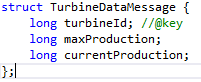
\includegraphics[width=0.3\textwidth,natwidth=250,natheight=200]{turbineDataMessage.PNG} 
	\captionsetup{format=plain,font=footnotesize,labelfont={bf,defaultCapFont},labelsep=quad,singlelinecheck=no}
	\caption[Centralized turbine reply message]{
		\label{fig:cenTurbineDataMessage} 
		\footnotesize{%
			The the reply message .idl file sent from the turbines to the Park Pilot in the centralized solution.
		}
	}
\end{figure}

The IDL definitions are are defined from looking at what data to transfer between the turbines and the Park Pilot. \Cref{fig:cenTurbineDataMessage} for example is IDL definition of the data transfer object used as reply from the turbines to the Park Pilot. 

\subsection{Topics}

Including the topics generated from the RTI Connext Request-Reply implementation~\cite{rtiConnextUsersManual} we are using the following topics:


%\begin{figure}
%	\centering
%	\begin{tikzpicture}[
	point/.style={inner sep=0pt}, %circle,minimum size=2pt,fill=red},
	textNode/.style={inner sep=2pt},
	hv path/.style={to path={-| (\tikztotarget)}},
	vh path/.style={to path={|- (\tikztotarget)}},
	skip loop h/.style={to path={-- ++(0,#1) -| (\tikztotarget)}},
	skip loop v/.style={to path={-- ++(#1,0) |- (\tikztotarget)}},
	graphs/every graph/.style={edges=rounded corners}
	]
	
% Place nodes
\matrix[row sep=1.4cm,column sep=.4cm] {
	\node [point]  		(p1x1)	{}; &&
	\node [rectangle]	(Turbine)		[draw, label=above:\textbf{$\cdot$}N Turbines, text width=50pt]	{Cur.Prod. Max.Prod}; &&
	\node [point]  		(p1x3)	{}; \\
	
	\node [point]  		(p2x1)			{}; &&
	\node [textNode]	(HPPP)		 	{Reg. algorithm}; &&
	\node [textNode]	(Setpoint)	{N Setpoints}; \\

	&& \node [textNode]  (gSetpoint)							{Global SetPoint}; \\
};
	
\graph[use existing nodes]{
	Turbine ->[skip loop v=-3.1cm] HPPP -> Setpoint ->[vh path] Turbine;
	gSetpoint -> HPPP;
};

\end{tikzpicture}



%\begin{tikzpicture}[
%	point/.style={inner sep=0pt}, %circle,minimum size=2pt,fill=red},
%	textNode/.style={inner sep=2pt},
%	hv path/.style={to path={-| (\tikztotarget)}},
%	vh path/.style={to path={|- (\tikztotarget)}},
%	skip loop h/.style={to path={-- ++(0,#1) -| (\tikztotarget)}},
%	skip loop v/.style={to path={-- ++(#1,0) |- (\tikztotarget)}},
%	graphs/every graph/.style={edges=rounded corners}
%	]
%	
%% Place nodes
%\matrix[row sep=1.5cm,column sep=.5cm] {
%	\node [point]  		(p1x1)	{}; &&
%	\node [rectangle]	(Turbine)		[draw, label=above:\textbf{$\cdot$}N Turbines, text width=50pt]	{Cur.Prod. Max.Prod}; &&
%	\node [point]  		(p1x3)	{}; \\
%	
%	\node [point]  		(p2x1)			{}; &&
%	\node [textNode]	(HPPP)		 	{HPPP}; &&
%	\node [textNode]	(Setpoint)	{\textbf{$\cdot$}N Setpoints}; \\
%
%	\node [textNode]  (gSetpoint)										{Global SetPoint}; &&
%	\node [rectangle]	(Data)			[draw, text width=50pt] {Cur.prod  Max.Prod};\\
%};
%
%\node [textNode,right of=Data] {~~~~~~~~~~~~~~~~~\textbf{$\cdot$}N Turbines};
%	
%\graph[use existing nodes]{
%	Turbine ->[skip loop v=-2.7cm] HPPP -> Setpoint ->[vh path] Turbine;
%	gSetpoint.east -> HPPP;
%	Data -> HPPP;
%};
%
%\end{tikzpicture}
%
%	\captionsetup{format=plain,font=footnotesize,labelfont={bf,defaultCapFont},labelsep=quad,singlelinecheck=no}
%	\caption[Regulation algorithm input/output parameters]{
%		\label{fig:ioRegAlg} 
%		\footnotesize{%
%			Input/output parameters of the regulation algorithm.
%		}
%	}
%\end{figure}

\subsection{Choosing QoS parameters}

Quality of service parameters are parameters used to determine system behavior. As such, setting the right ones for our system is important in order to get the centralized solution to behave as much as the current system at Siemens as possible. 

In order to decide the QoS parameters for the centralized, the QoS XML file from the current system at Siemens was provided by Siemens (see \cref{appendix:siemensQosFile} for the QoS XML file). Thus QoS parameters for the centralized solution has been set using this file, which presents many different QoS profiles.

The Siemens QoS XML file (\cref{appendix:siemensQosFile}) only specifies one participant factory profile and one participant profile. Both profiles has applied to the solution and only parameters irrelevant to the purpose of this thesis has been removed from the profiles. 

However, the file specifies many different profiles for DataReaders, DataWriters and Topics and where each profile has been applied to the current system at Siemens has not been informed by Siemens. Thus we don't know which ones has been used for the part of the system that is implemented with the centralized solution. 

Each parameter in every QoS profile has been evaluated and the parameters relevant to the purpose of this theses has been applied to the centralized solution, based on assumptions about the current Siemens system. The QoS XML file roughly presents profiles that combines the following parameters in different ways:

\paragraph{Reliability} is the parameter, which determines whether or not data published by a DataWriter will be reliably delivered by the DDS framework to matching DataReaders~\cite{rtiConnextUsersManual}. The three levels of reliability presented by the different profiles are:

\begin{itemize}
	\item \textbf{Best effort reliability} profiles are configured so data samples are sent once and missed samples are acceptable.
	\item \textbf{Reliable} profiles are configured to make sure that data sent is received and missed samples are resent. DataWriters will send samples reliably to DataReaders, buffering sent data until they have been acknowledged as being received by DataReaders and resending any samples that may have been lost during transport. The DataWriter buffer of this configuration is set to the size of one message, which means only the newest message are resent. This implies that an unacknowledged sample may be overwritten and thus lost. 
	\item \textbf{Strictly reliable} profiles are configured exactly like reliable profiles, but with a larger DataWriter buffer. Increasing the DataWriter buffer size will decrease the chance of unacknowledged samples being overwritten. Thus DataReaders are ensured all messages sent by the DataWriters.
\end{itemize}

\paragraph{Durability} controls whether or not, and how, published samples are stored by the DataWriter application for DataReaders that are found after the samples were initially written, thus allowing new DataReaders to receive data sent before they were created. The levels of durability presented by the different profiles are:

\begin{itemize}
	\item \textbf{No durability} profiles are configured not to store any samples for newly discovered DataReaders.
	\item \textbf{Local durability} profiles are configured so that DataWriters will store and send previously published samples for delivery to newly discovered DataReaders as long as the DataWriter still exists.
\end{itemize}

\paragraph{Throughput} is configured using the batch~\cite{rtiConnextUsersManual} parameter, which can be used to decrease the amount of communication overhead associated with the transmission and (in case of reliable communication) acknowledgment of small samples at the expense of latency. This is done by batching many smaller samples to be sent in a single large packet, which increases network utilization and thus throughput in terms of samples per second. The two levels of throughput presented by the different profiles are:

\begin{itemize}
	\item \textbf{Regular throughout} profiles are configured not batch any samples, thus data samples and (in case of reliable communication) acknowledgment message are sent individually.
	\item \textbf{High throughput} profiles are configured so DataWriters will batch data in order to increase throughput.
\end{itemize}

The many profiles in the Siemens QoS XML file (\cref{appendix:siemensQosFile}) are presumably made for many different purposes. For building the centralized solution, the profile using \textbf{Strictly reliable}, \textbf{No durability} and \textbf{Regular throughput} configurations was chosen based on the following assumptions about the current Siemens system:

\begin{itemize}
	\item \textbf{Strictly reliable} messaging is important for the Park Pilot to compute setpoints for each turbine, since states of all turbines are needed in order to calculate setpoints. Thus resending a sample data if the sample data is dropped is needed in order to calculate setpoints. 
	\item \textbf{No durability} is needed for the regulation algorithm. If a new turbine is discovered, the turbine have no need of receiving old requests or setpoints. The turbine only needs to make itself available to requests from the Park Pilot and thereby be taken into account, which is done automatically by \textit{Connext} when a new DataReader is discovered.  
	\item \textbf{Regular throughput} provides the best performance for the regulation cycle. Batching data samples and potentially end in a situation where two turbine states are returned to the regulation algorithm bundled is not acceptable. 
\end{itemize}

All parameters of the quality of service configuration for the centralized solution is presented and described in section \cref{sec:detailedQoSDesc}.


\subsection{Detailed QoS evaluation} \label{sec:detailedQoSDesc}
\lstset{tabsize=2, language=XML, basicstyle=\small}

The section provides a detailed evaluation of every parameter of the centralized solution QoS XML file, including the QoS parameters deemed irrelevant and thereby removed from the QoS file provided by Siemens (\cref{appendix:siemensQosFile}). Removed parameters are marked with '(Removed)'.

\paragraph{Logging} every time an error occurs (\cref{fig:parFacLogQos})


\begin{figure}
\begin{lstlisting}
<participant_factory_qos>
    <logging>
        <verbosity>WARNING</verbosity>
        <category>PLATFORM</category>
        <print_format>VERBOSE_TIMESTAMPED</print_format>
        <output_file>ddsadaptor.log</output_file>
    </logging>
</participant_factory_qos>
\end{lstlisting}
\caption[Participant factory logging QoS]{
		\label{fig:parFacLogQos} 
		\footnotesize{Participant factory logging QoS.}
	}
\end{figure}


%DTLS --> underlying UDP, multicast disabled

%<autoenable_created_entities>false</autoenable_created_entities> we default should be true. We don't need any disabled entities

%logging: removed from both systems
%discovery
%buffer size
%participant, UDP, dtls
%datareader, liveliness, best effort reliability, history 1
%datawriter, liveliness, same as reader, heartbeat watermarks for reliability

%Siemens er ved at skifte til, UDP Det giver mere mening, sparer netværks trafik


\section{Theoretical comparison to the existing system at Siemens Wind Power}
